\documentclass[a4paper,11pt]{scrartcl}
\usepackage{listings}
\usepackage{setspace}
\usepackage{color}
\usepackage{sansmathfonts}
\usepackage{helvet}
\usepackage{amsmath,amssymb,amsthm, mathtools} 
\usepackage{algpseudocode}

\newtheorem{theorem}{Theorem}
\newtheorem{lemma}{Lemma}
\renewcommand{\familydefault}{\sfdefault}
\onehalfspacing

\begin{document}
\newcommand{\operation}[2]{\textsc{#1}($#2$)}

\section{Question 1}
\subsection{Part (a)}
To implement \textsc{Decrement}:

\begin{algorithmic}[1]

\Function{Decrement}{$A$, $k$}
    \State $i \gets 0$
    \While{ $i < k \land A_i = 0$ }
        \State $A_i \gets 1$
        \State $i \gets i+1$
    \EndWhile
    \If{$i < k$}
        \State $A_i \gets 0$
    \EndIf
\EndFunction

\end{algorithmic}

To achieve an $\Omega(k)$ average operation cost, on a $k$-bit counter that initially contains $x$ ($0 \leq x < 2^k$), supposing that each change of a value in $A$ has unit cost, there are 2 cases:

\begin{itemize}
    \item $x = 0$: In this case, do a single \textsc{Decrement} operation. The cost for this operation is $k$ (as it will set all $k$ bits of the counter to 1), and thus, the average cost for the operation is also $k$ i.e. is $\Omega(k)$.
    \item $x > 0$: First do $x$ \textsc{Decrement} operations (setting the counter to $0$), and then alternate \textsc{Decrement} and \textsc{Increment} $x$ times. The first $x$ operations cost at least $1$ each, whereas the next $x$ operations (which consist either of \textsc{Decrement}-ing a counter that contains $0$, or \textsc{Increment}-ing a counter that contains $2^k-1$) each have cost $k$. Thus the average cost per operation is at least $\frac{x + x k}{2 x} = \frac{k + 1}{2}$ i.e. is $\Omega(k)$.
\end{itemize}

\subsection{Part (b)}
To efficiently implement \textsc{Reset}, while using only $k$ extra bits, maintain another array of bits $B[0..k)$ that satisfies the following invariant:
\begin{center}
    $B_i = A_i \lor A_{i+1} \lor ... \lor A_{k-1}$
\end{center}

$B$ will thus initially contain only 0's. Now to see the effects of the various operations. \\
An \textsc{Increment} operation will set a bit in $B$ to 1 whenever a corresponding bit in $A$ is set to 1. Also, when an \textsc{Increment} overflows the counter, $B$ is set entirely to $0$:

\begin{algorithmic}[1]
\Function{Increment}{$A$, $B$, $k$}
    \State  $i \gets 0$
    \While{ $i < k \land A_i = 1$ }
        \State $A_i \gets 0$
        \State $i \gets i+1$
    \EndWhile
    \If{$i < k$}
        \State $A_i \gets 1$
        \State $B_i \gets 1$
    \Else
        \While{ $i \geq 0$}
            \State $B_i \gets 0$
            \State $i \gets i-1$
        \EndWhile
    \EndIf
\EndFunction
\end{algorithmic}

To implement \textsc{Reset}, use the array $B$ to decide "how far" to go in $A$ when setting bits to 0. This works since, once $B$ becomes 0, by the invariant, $A$ will have no further bits to reset:

\begin{algorithmic}[1]
\Function{Reset}{$A$, $B$, $k$}
    \State $i \gets 0$
    \While { $i < k \land B_i = 1$ }
        \State $A_i \gets 0$
        \State $B_i \gets 0$
        \State $i \gets i+1$
    \EndWhile
\EndFunction
\end{algorithmic}

To show that this has amortized $O(1)$ complexity, assuming that each operation that sets a value in $A$ or $B$ has unit cost, consider the following potential function on the state of the data structure:

\begin{center}
$\Phi(A, B, k) \coloneqq f_1(A) + 2 f_1(B)$
\end{center}

Where $f_1(X)$ represents the number of times the bit 1 appears in an array $X$. This is a valid potential function since it is initially zero, and is by definition always non-negative and real.

I now analyse each operation's cost separately:

\begin{itemize}
    \item \textsc{Increment}: Here there are two cases:
        \begin{itemize}
            \item If no overflow occurs, suppose that $x$ bits are set to $0$ in lines 3-6. Since no overflow occurs, we enter the \textbf{if} on lines 7-10, not the \textbf{else} on lines 10-14. Thus, we do $x + 2$ actual operations; however, the potential is reduced by $x$ by lines 3-6, and increased by 3 on lines 7-10. We thus have an amortized cost of $x + 2 - x + 3 = 5$ i.e. $O(1)$.
            \item If overflow occurs, then lines 3-6 will set $k$ bits to $0$. Since overflow occurs, we enter the \textbf{else} on lines 10-14, not the \textbf{if} on lines 7-10. Thus we do a further $k$ operations in setting all bits of $B$ to $0$. However, the potential is reduced by $k$ by lines 3-6 and by a further $2k$ by lines 10-14. Thus the amortized cost of the operation in this case is $k + k - k - 2k = -k \leq 0$ i.e. $O(1)$.
        \end{itemize}
    \item \textsc{Reset}: Here, suppose the \textbf{while} on lines 3-6 runs $x$ times. We thus do $2 x$ actual operations. On the other hand, each iteration will certainly set a bit in $B$ from 1 to 0, reducing the potential by 2. While we may also reduce the potential by setting a bit in $A$ from 1 to 0, this will not necessarily happen on every iteration. Thus, the potential is reduced by at least $2 x$, leading us to an amortized cost of at most $2x - 2x = 0$ i.e. $O(1)$.
\end{itemize}

So, in all cases, we have an $O(1)$ amortized cost per operation.

\section{Question 2}

To implement such a data structure, allocate two stacks $A$ and $B$ that support operations \textsc{Pop}, \textsc{Push} and \textsc{Empty}, where the \textsc{Pop} operation not only removes the top element from a stack, but also returns it. I assume these to take unit time. I also assume that \textsc{Dequeue} is required not only to remove an element from the queue, but also return it. Thus, implement \textsc{Enqueue} and \textsc{Dequeue} as follows:

\begin{algorithmic}[1]
\Function{Enqueue}{$A, B, x$}
    \State \textsc{Push}($A, x$)
\EndFunction

\Function{Dequeue}{$A, B, x$}
    \If{\textsc{Empty}($B$)}
        \While{$\lnot$ \textsc{Empty}($A$)}
            \State \textsc{Push}($B$, \textsc{Pop}($A$))
        \EndWhile
    \EndIf
    \State \Return \textsc{Pop}($B$)
\EndFunction
\end{algorithmic}

To see why this is correct, note that if our data structure represents a queue which holds a sequence $S$ (where we \textsc{Enqueue} to the front of $S$ and \textsc{Dequeue} from the back of $S$), then $S = \langle A \rangle \Vert reverse\langle B \rangle$, where $\langle X \rangle$ represents the contents of some stack $X$ taken from top to bottom, and $\Vert$ represents concatenation. With this in mind, note that \textsc{Enqueue} inserts $x$ to the top of $A$, thus indeed putting $x$ at the beginning of $S$. \textsc{Dequeue} may initially, if $B$ is empty, set $B$ to $reverse(A)$ and erase all elements from $A$ (which overall does not change $S$, as $S$ is initially $\langle A \rangle \Vert \epsilon$, and after this it is $\epsilon \Vert reverse (reverse \langle A \rangle )$, where $\epsilon$ is the empty sequence -- and these two sequences are equal) after which it returns the element at the top of $B$, which indeed represents the last element of $S$. \\
To show that this data structure has $O(1)$ amortized complexity for either operation, consider the following potential function:

$\Phi(A, B) \coloneqq |A|$

Where $|A|$ is the size of $A$. \\
I now show that each operation in turn has $O(1)$ amortized complexity:

\begin{itemize}
    \item \textsc{Enqueue}: Here we do 1 actual operation, and increase $\Phi(A, B)$ by 1. So the amortized cost is $2$ i.e. $O(1)$.
    \item \textsc{Dequeue}: There are 2 cases:
        \begin{itemize}
            \item if the \textbf{if} on line 5 is triggered, we do $|A|$ operations in the \textbf{while} on lines 6-8. Additionally we do 1 further operation on line 10. On the other hand, the \textbf{while} also reduces the potential by $|A|$, since it empties stack $A$, which leads to an amortized cost of $|A| + 1 - |A| = 1$ i.e. $O(1)$.
            \item otherwise, we only do the 1 operation on line 10, and we do not modify the potential, so the amortised cost is $O(1)$.
        \end{itemize}
\end{itemize}

So overall the data structure has $O(1)$ amortised time complexity.

\section{Question 3}

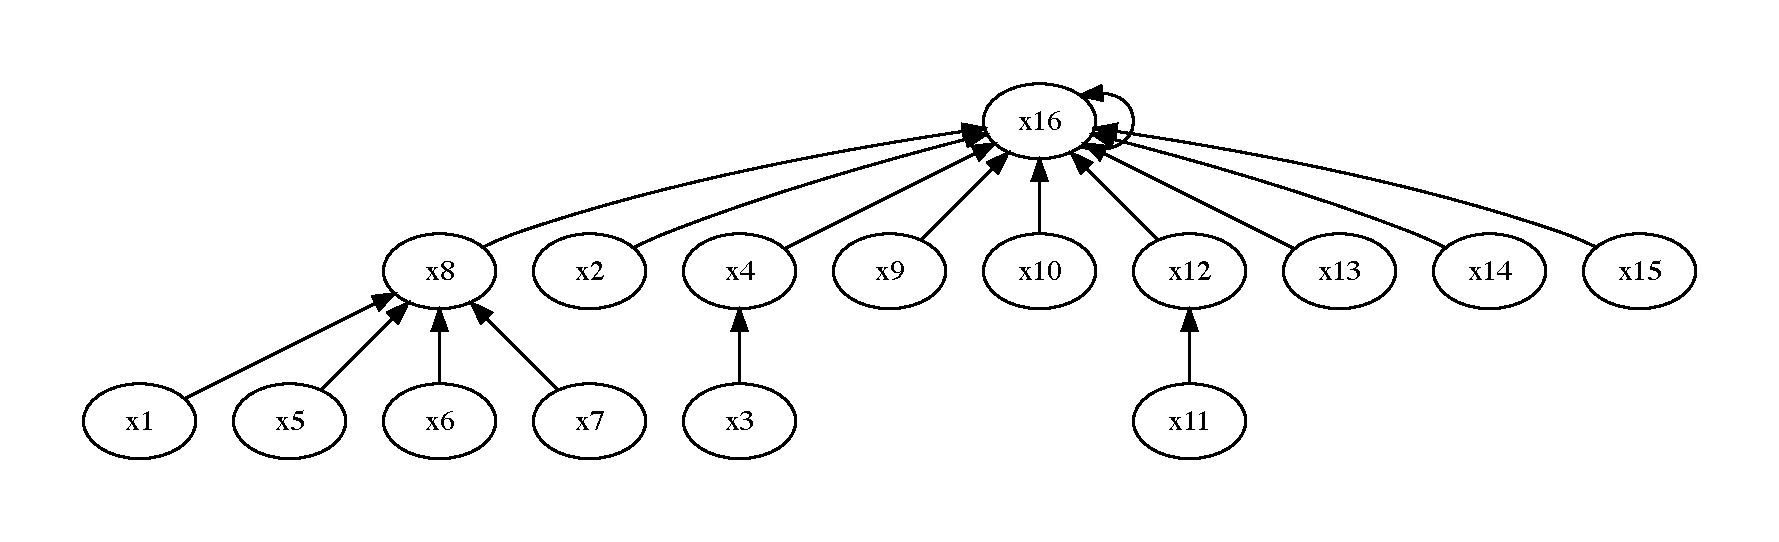
\includegraphics[width=\textwidth]{diagram.pdf}

\section{Question 4}

Note that: \\
    $log(n) = log(65536^{65536^{65536}}) = log(2^{16 * 65536^{65536}}) = 16 * 65536 ^ {65536}$ \\
    $log(log(n)) = log(16 * 65536 ^ {65536}) = 4 + log(2 ^ {4 * 65536}) = 4 + 4 * 65536$ \\
    $log(log(log(n))) = log(4 + 4 * 65536) \approx 18.00002$ \\
    $log(log(log(log(n)))) \approx log(18.00002) \approx 4.169$ \\
    $log(log(log(log(log(n))))) \approx 2.059$ \\
    $log(log(log(log(log(log(n)))))) \approx 1.042$ \\
    $log(log(log(log(log(log(log(n))))))) \approx 0.059$ \\
This implies that $log^*(n) = 7$.

\section{Question 5}
To show this, take $n = 2^k$, for any $k \in \mathbb{N}$, and let $m$ be equal to $2n - 1$. Now use the following operations on initial values $1 ... n$: \\

\begin{algorithmic}
\For{$i \gets 1 ... k$}
    \For{$j \gets 2^{i-1} ... n - 2^{i-1} \textbf{ step } 2^i$}
        \State \operation{Union}{j, j + 2^{i-1}}
    \EndFor
    \State \Comment{after this, nodes $2^i, 2 * 2^i, 3 * 2^i, ..., n$ have subtree height $i$}
\EndFor
\State \Comment{Now, $n$ has subtree height $k = log_2(n)$, and we have done $n-1$ operations so far. Note also, that at this point, $1$ is a leaf at depth $k = log_2(n)$}

\For{$i \gets 1 ... n$}
    \State \operation{Find}{1}
\EndFor
\end{algorithmic}

Now note that:
\begin{itemize}
    \item There are $n - 1$ \textsc{Union}'s, but, for the purpose of this analysis, we can ignore their cost. This is valid as we are asked to prove a lower bound on the total cost.
    \item We use $n$ \textsc{Find} operations, and each takes time proportional to the depth of node $1$ i.e. $log_2(n)$. Since, again, $m = 2n - 1$, this implies that we use $\Omega(m\ log_2(n))$ time for these operations.
\end{itemize}
This means that we use $\Omega(m\ log(n))$ time overall.
\end{document}
